\section{Implementation, Integration and Test Plan}

As it was already presented in the previous Sections, the System can be seen in terms of three main subsystems:
\begin{itemize}
\item \textbf{Front-end subsystem}: Report Manager, Encryption Manager, Network Manager, Presentation.
\item \textbf{Back-end subsystem}: Authentication Manager, Authority Manager, User Manager, Report Manager, Ticket Manager, Network Manager, Encryption Manager, Data Store Manager, Data Manager, Suggestion Manager, Statistics Manager, Urban Safeness Manager, Database.
\item \textbf{External subsystem}: Mailing Service, GPS, Map Service, Municipality System, Authority Ticket Service, License Plate Recognition API, Corrupted Image Recognition API. 
\end{itemize}
The implementation, integration and testing of the System will follow a \textit{bottom-up} approach, without leaving aside the dependencies between components in the same subsystem. Thus, the implementation and integration process will begin considering  different components in the same subsystem as first step and then it will continue with the integration of different subsystems.\newline
It is important to notice that components in the external subsystem do not need to be implemented and tested since it is assumed that they are reliable.\newline
Another crucial fact to be considered is that, besides following a \textit{bottom-up} approach, it is possible to implement components in parallel by using an incremental approach for the integration and testing processes. Once two components  (within the same subsystem) are implemented, the integration and testing of those can be performed.
\subsection{Implementation Plan}
The implementation order each component in the Server side shall be:
\begin{enumerate}
    \item Database Services (Database, Data Storage Manager)
    \item Encryption Manager and Network Manager
    \item Account Services (Authentication Manager, User Manager, Authority Manager)
    \item Traffic Ticket Services (Report Manager, Ticket Manager)
    \item Supplementary Services (Data Manager, Suggestions Manager, Statistics Manager, Urban Safeness Manager)
\end{enumerate}
In the Database Services, since Data Storage Manager uses the Database, the idea of the \textit{bottom-up} approach is to implement first the basic structure of the Database (and to chose the DBMS). Once the Database has been implemented, the Data Storage Manager can be implemented.\newline
Network Manager and Encryption Manager are used to allow a secure communication between external services and internal services, and since it is important for the integration of the subsystems and components, it should be implemented as soon as the Database Services are working and we are able to receive/send messages.\newline
Account Services allows to manage all the information about Users and what functionalities they can access, thus, this set of components should be implemented before Traffic Ticket Services.\newline
Traffic Ticket Services are crucial for the basic functionalities of SafeStreets, thus, these components should be implemented before the Supplementary components.\newline
The implementation order of each component in the client application side shall be:
\begin{enumerate}
	\item Encryption Manager and Network Manager
	\item Report Manager
	\item Presentation
\end{enumerate}
Following the \textit{bottom-up} approach the Presentation component will be implemented as the last component in the client application side since it will need to use Report Manager, Ticket Manager, Encryption Manager and Network Manager.
\subsection{Integration and Test Plan}
In the following diagrams it will be shown how the integration and testing are performed. Network Manager and Encryption Manager will not be included for readability purposes, but it should be kept in mind that their integration and testing are performed after the components of the Database Services have been integrated and tested. Before starting with the integration process, all the unit test for each component already implemented will be performed. Once the unit test phase have been completed, the integration process can start.
\subsubsection{Integration Process}
Following what have been said in the previous section, the integration process follows an incremental approach, when a set of components (in the same Service) have been implemented, their integration will be performed.\\\\
\textbf{Integration of components inside the Database Services }\newline
The first set of components to be integrated and tested are the ones that interact with the Database, thus, once the implementation of the Database have been completed its integration and testing with the Data Store Manager should begin.
     \begin{figure}[H]
     \centering
          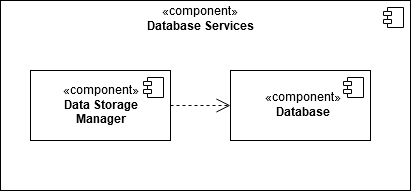
\includegraphics[width=0.6\textwidth]{Images/db_services_definitivo.png}
        \caption{Integration of Database Services}
    \end{figure}
            \noindent\textbf{Integration of components inside the Account Services }\newline
This set contains the components that allows to identify and authenticate a user. Once the User Manager and Authority Manager have been implemented and the unit testing of each have been performed, they can be integrated with the Authentication Manager.
     \begin{figure}[H]
         \centering
          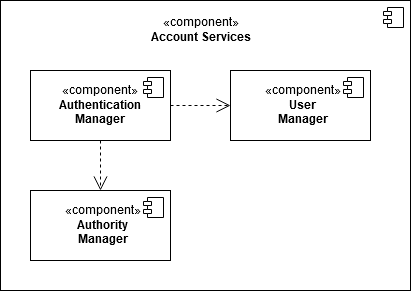
\includegraphics[width=0.6\textwidth]{Images/account_service.png}
        \caption{Integration of Account Services}
    \end{figure}
\noindent\textbf{Integration of components inside the Traffic Ticket Services }\newline
This set of components contains the Report Manager and the Ticket Manager, the first component that has been implemented is Ticket Manager since it is used by the Report Manager, once the implementation of Ticket Manager and Report Manager have been completed their integration and testing will start.
     \begin{figure}[H]
         \centering
          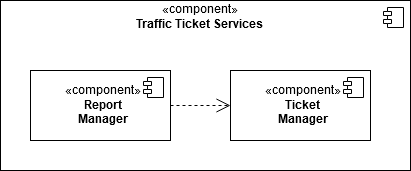
\includegraphics[width=0.6\textwidth]{Images/tt_services.png}
        \caption{Integration of Traffic Ticket Services}
    \end{figure}

    \noindent\textbf{Integration of components inside the Supplementary Services }\newline
    Once the components that allows to perform the basic functionalities have been integrated and tested, the same process should be performed for the components that contains the logic behind the supplementary services. Following the \textit{bottom-up} approach, once the leaves in the use hierarchy are ready to be integrated, the integration with Data Manager can start.
         \begin{figure}[H]
             \centering
          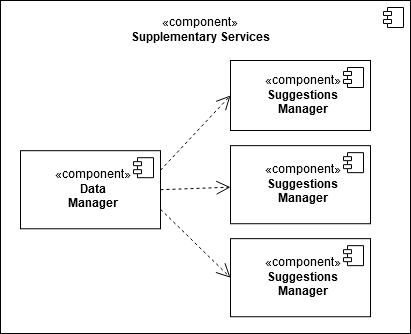
\includegraphics[width=0.6\textwidth]{Images/supplementary_services.png}
        \caption{Integration of Supplementary Services}
    \end{figure}

    \noindent\textbf{Integration of services inside the Back-end Subsystem}\newline
Once all the components inside the application server have been implemented, integrated and tested, the last integration and test can be performed and, thus, the back-end part will be ready to interact with the the client application.
    
         \begin{figure}[H]
             \centering
      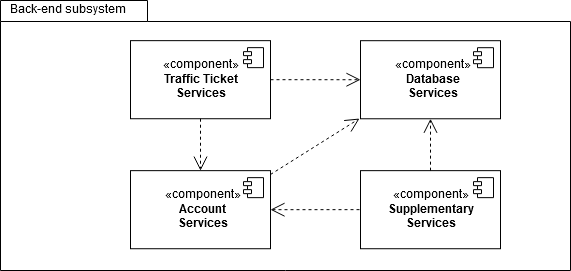
\includegraphics[width=1\textwidth]{Images/back_end_definitivo.png}
        \caption{Integration of the Back-end Subsystem}
    \end{figure}
\vspace{2mm}
\noindent\textbf{Integration of components inside the Front-end Subsystem}\newline
Since the Front-end subsystem contains only the Encryption Manager, Network Manager, Report Manager and Presentation components, and three of the four components were already present in the back-end subsystem (for Report Manager different logic but same purpose), their integration and test process will be the same with the only difference that the Presentation component will be the last component to be integrated and tested. In the following diagrams, the front-end subsystem will be represented as the \noindent\textit{Client Application} component.\newline \\
The following two diagrams represents how the integration between the client application and the application server is performed. First the client application is integrated and tested with the basic functionalities (Traffic Ticket Services), and then with the additional functionalities (Supplementary Services). At the end of each integration, an integration test is performed.
\begin{figure}[H]
             \centering
          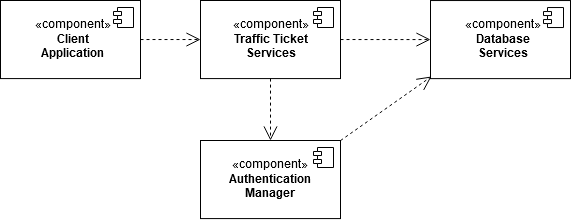
\includegraphics[width=0.8\textwidth]{Images/client_tt_services.png}
        \caption{Client Application with Traffic Ticket Services}
        
    \end{figure}
         \begin{figure}[H]
             \centering
          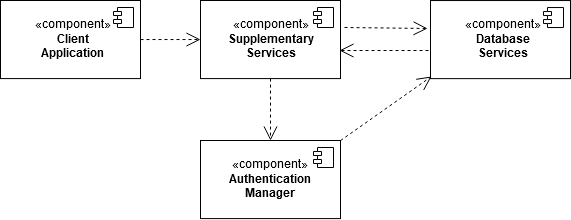
\includegraphics[width=0.8\textwidth]{Images/client_supp_services.png}
        \caption{Client Application with Supplementary Services}
    \end{figure}